\chapter{Grid Search}
\label{ch4}

\section{Methodology}

\section{Results}
\begin{figure}[h!]
	\centering
	\subfloat[Full set of iterations\label{fig:grid_search_results_a}]{
		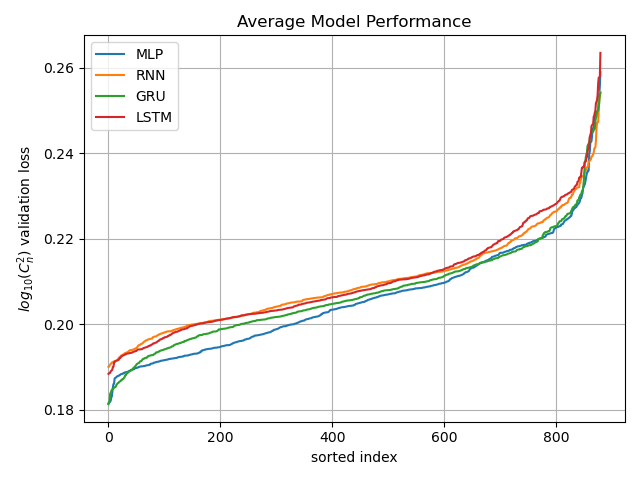
\includegraphics[width=0.49\textwidth]{average_model_performance_wide.png}
	}
	\subfloat[Top 10 iterations\label{fig:grid_search_results_b}]{
		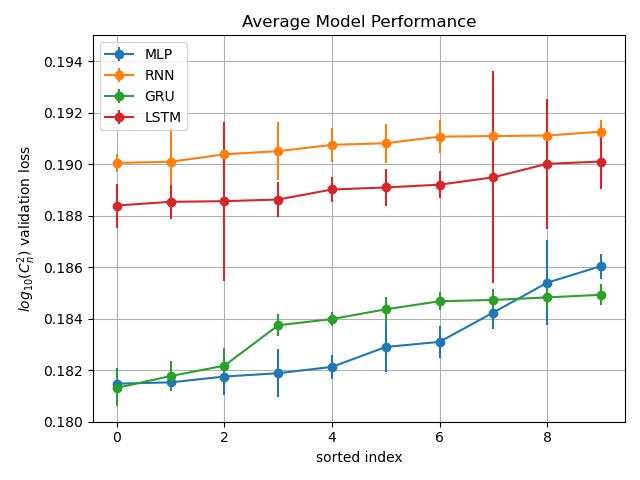
\includegraphics[width=0.49\textwidth]{average_model_performance_narrow.png}
	}
	\hfill
	\caption{Grid search results.}
	\label{fig:grid_search_results}
\end{figure}

\begin{figure}[h!]
	\centering
	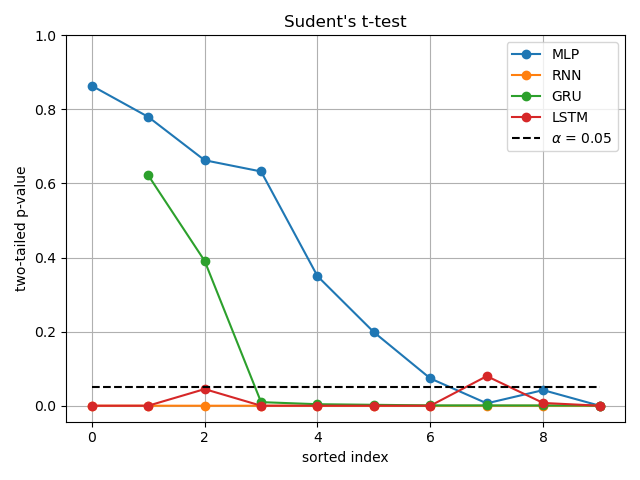
\includegraphics[width=0.65\textwidth]
	{students_t-test.png}
	\hfill
	\caption{Grid search results.}
	\label{fig:students_t-test}
\end{figure}

\begin{figure}[h!]
	\centering
	\subfloat[Best 10\%\label{fig:variable_sets_analysis_a}]{
		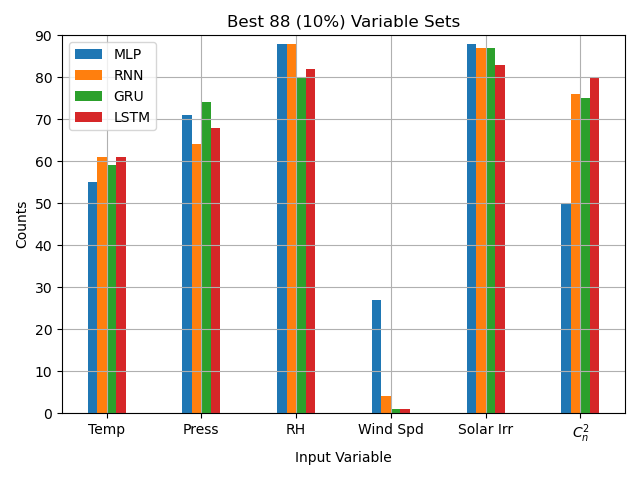
\includegraphics[width=0.49\textwidth]{bar_variable_sets_best.png}
	}
	\subfloat[Worst 10\%\label{fig:variable_sets_analysis_b}]{
		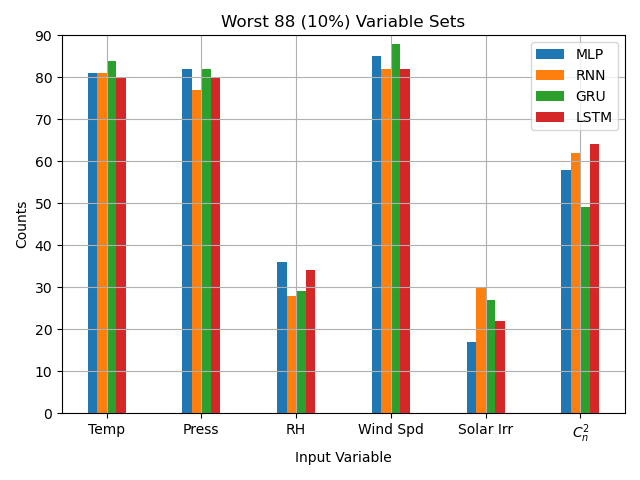
\includegraphics[width=0.49\textwidth]{bar_variable_sets_worst.png}
	}
	\hfill
	\caption{Best 10\% and worst 10\% variable sets.}
	\label{fig:variable_sets_analysis}
\end{figure}